
% Default to the notebook output style




% Inherit from the specified cell style.





\documentclass{article}



    \usepackage{graphicx} % Used to insert images
    \usepackage{adjustbox} % Used to constrain images to a maximum size
    \usepackage{color} % Allow colors to be defined
    \usepackage{enumerate} % Needed for markdown enumerations to work
    \usepackage{geometry} % Used to adjust the document margins
    \usepackage{amsmath} % Equations
    \usepackage{amssymb} % Equations
    \usepackage{eurosym} % defines \euro
    \usepackage[mathletters]{ucs} % Extended unicode (utf-8) support
    \usepackage[utf8x]{inputenc} % Allow utf-8 characters in the tex document
    \usepackage{fancyvrb} % verbatim replacement that allows latex
    \usepackage{grffile} % extends the file name processing of package graphics
                         % to support a larger range
    % The hyperref package gives us a pdf with properly built
    % internal navigation ('pdf bookmarks' for the table of contents,
    % internal cross-reference links, web links for URLs, etc.)
    \usepackage{hyperref}
    \usepackage{longtable} % longtable support required by pandoc >1.10
    \usepackage{booktabs}  % table support for pandoc > 1.12.2




    \definecolor{orange}{cmyk}{0,0.4,0.8,0.2}
    \definecolor{darkorange}{rgb}{.71,0.21,0.01}
    \definecolor{darkgreen}{rgb}{.12,.54,.11}
    \definecolor{myteal}{rgb}{.26, .44, .56}
    \definecolor{gray}{gray}{0.45}
    \definecolor{lightgray}{gray}{.95}
    \definecolor{mediumgray}{gray}{.8}
    \definecolor{inputbackground}{rgb}{.95, .95, .85}
    \definecolor{outputbackground}{rgb}{.95, .95, .95}
    \definecolor{traceback}{rgb}{1, .95, .95}
    % ansi colors
    \definecolor{red}{rgb}{.6,0,0}
    \definecolor{green}{rgb}{0,.65,0}
    \definecolor{brown}{rgb}{0.6,0.6,0}
    \definecolor{blue}{rgb}{0,.145,.698}
    \definecolor{purple}{rgb}{.698,.145,.698}
    \definecolor{cyan}{rgb}{0,.698,.698}
    \definecolor{lightgray}{gray}{0.5}

    % bright ansi colors
    \definecolor{darkgray}{gray}{0.25}
    \definecolor{lightred}{rgb}{1.0,0.39,0.28}
    \definecolor{lightgreen}{rgb}{0.48,0.99,0.0}
    \definecolor{lightblue}{rgb}{0.53,0.81,0.92}
    \definecolor{lightpurple}{rgb}{0.87,0.63,0.87}
    \definecolor{lightcyan}{rgb}{0.5,1.0,0.83}

    % commands and environments needed by pandoc snippets
    % extracted from the output of `pandoc -s`
    \DefineVerbatimEnvironment{Highlighting}{Verbatim}{commandchars=\\\{\}}
    % Add ',fontsize=\small' for more characters per line
    \newenvironment{Shaded}{}{}
    \newcommand{\KeywordTok}[1]{\textcolor[rgb]{0.00,0.44,0.13}{\textbf{{#1}}}}
    \newcommand{\DataTypeTok}[1]{\textcolor[rgb]{0.56,0.13,0.00}{{#1}}}
    \newcommand{\DecValTok}[1]{\textcolor[rgb]{0.25,0.63,0.44}{{#1}}}
    \newcommand{\BaseNTok}[1]{\textcolor[rgb]{0.25,0.63,0.44}{{#1}}}
    \newcommand{\FloatTok}[1]{\textcolor[rgb]{0.25,0.63,0.44}{{#1}}}
    \newcommand{\CharTok}[1]{\textcolor[rgb]{0.25,0.44,0.63}{{#1}}}
    \newcommand{\StringTok}[1]{\textcolor[rgb]{0.25,0.44,0.63}{{#1}}}
    \newcommand{\CommentTok}[1]{\textcolor[rgb]{0.38,0.63,0.69}{\textit{{#1}}}}
    \newcommand{\OtherTok}[1]{\textcolor[rgb]{0.00,0.44,0.13}{{#1}}}
    \newcommand{\AlertTok}[1]{\textcolor[rgb]{1.00,0.00,0.00}{\textbf{{#1}}}}
    \newcommand{\FunctionTok}[1]{\textcolor[rgb]{0.02,0.16,0.49}{{#1}}}
    \newcommand{\RegionMarkerTok}[1]{{#1}}
    \newcommand{\ErrorTok}[1]{\textcolor[rgb]{1.00,0.00,0.00}{\textbf{{#1}}}}
    \newcommand{\NormalTok}[1]{{#1}}

    % Define a nice break command that doesn't care if a line doesn't already
    % exist.
    \def\br{\hspace*{\fill} \\* }
    % Math Jax compatability definitions
    \def\gt{>}
    \def\lt{<}
    % Document parameters
    \title{Converting  Vehicles To Number Of Shoppers}
    \author{Daniel Cuneo}




    % Pygments definitions

\makeatletter
\def\PY@reset{\let\PY@it=\relax \let\PY@bf=\relax%
    \let\PY@ul=\relax \let\PY@tc=\relax%
    \let\PY@bc=\relax \let\PY@ff=\relax}
\def\PY@tok#1{\csname PY@tok@#1\endcsname}
\def\PY@toks#1+{\ifx\relax#1\empty\else%
    \PY@tok{#1}\expandafter\PY@toks\fi}
\def\PY@do#1{\PY@bc{\PY@tc{\PY@ul{%
    \PY@it{\PY@bf{\PY@ff{#1}}}}}}}
\def\PY#1#2{\PY@reset\PY@toks#1+\relax+\PY@do{#2}}

\expandafter\def\csname PY@tok@gd\endcsname{\def\PY@tc##1{\textcolor[rgb]{0.63,0.00,0.00}{##1}}}
\expandafter\def\csname PY@tok@gu\endcsname{\let\PY@bf=\textbf\def\PY@tc##1{\textcolor[rgb]{0.50,0.00,0.50}{##1}}}
\expandafter\def\csname PY@tok@gt\endcsname{\def\PY@tc##1{\textcolor[rgb]{0.00,0.27,0.87}{##1}}}
\expandafter\def\csname PY@tok@gs\endcsname{\let\PY@bf=\textbf}
\expandafter\def\csname PY@tok@gr\endcsname{\def\PY@tc##1{\textcolor[rgb]{1.00,0.00,0.00}{##1}}}
\expandafter\def\csname PY@tok@cm\endcsname{\let\PY@it=\textit\def\PY@tc##1{\textcolor[rgb]{0.25,0.50,0.50}{##1}}}
\expandafter\def\csname PY@tok@vg\endcsname{\def\PY@tc##1{\textcolor[rgb]{0.10,0.09,0.49}{##1}}}
\expandafter\def\csname PY@tok@m\endcsname{\def\PY@tc##1{\textcolor[rgb]{0.40,0.40,0.40}{##1}}}
\expandafter\def\csname PY@tok@mh\endcsname{\def\PY@tc##1{\textcolor[rgb]{0.40,0.40,0.40}{##1}}}
\expandafter\def\csname PY@tok@go\endcsname{\def\PY@tc##1{\textcolor[rgb]{0.53,0.53,0.53}{##1}}}
\expandafter\def\csname PY@tok@ge\endcsname{\let\PY@it=\textit}
\expandafter\def\csname PY@tok@vc\endcsname{\def\PY@tc##1{\textcolor[rgb]{0.10,0.09,0.49}{##1}}}
\expandafter\def\csname PY@tok@il\endcsname{\def\PY@tc##1{\textcolor[rgb]{0.40,0.40,0.40}{##1}}}
\expandafter\def\csname PY@tok@cs\endcsname{\let\PY@it=\textit\def\PY@tc##1{\textcolor[rgb]{0.25,0.50,0.50}{##1}}}
\expandafter\def\csname PY@tok@cp\endcsname{\def\PY@tc##1{\textcolor[rgb]{0.74,0.48,0.00}{##1}}}
\expandafter\def\csname PY@tok@gi\endcsname{\def\PY@tc##1{\textcolor[rgb]{0.00,0.63,0.00}{##1}}}
\expandafter\def\csname PY@tok@gh\endcsname{\let\PY@bf=\textbf\def\PY@tc##1{\textcolor[rgb]{0.00,0.00,0.50}{##1}}}
\expandafter\def\csname PY@tok@ni\endcsname{\let\PY@bf=\textbf\def\PY@tc##1{\textcolor[rgb]{0.60,0.60,0.60}{##1}}}
\expandafter\def\csname PY@tok@nl\endcsname{\def\PY@tc##1{\textcolor[rgb]{0.63,0.63,0.00}{##1}}}
\expandafter\def\csname PY@tok@nn\endcsname{\let\PY@bf=\textbf\def\PY@tc##1{\textcolor[rgb]{0.00,0.00,1.00}{##1}}}
\expandafter\def\csname PY@tok@no\endcsname{\def\PY@tc##1{\textcolor[rgb]{0.53,0.00,0.00}{##1}}}
\expandafter\def\csname PY@tok@na\endcsname{\def\PY@tc##1{\textcolor[rgb]{0.49,0.56,0.16}{##1}}}
\expandafter\def\csname PY@tok@nb\endcsname{\def\PY@tc##1{\textcolor[rgb]{0.00,0.50,0.00}{##1}}}
\expandafter\def\csname PY@tok@nc\endcsname{\let\PY@bf=\textbf\def\PY@tc##1{\textcolor[rgb]{0.00,0.00,1.00}{##1}}}
\expandafter\def\csname PY@tok@nd\endcsname{\def\PY@tc##1{\textcolor[rgb]{0.67,0.13,1.00}{##1}}}
\expandafter\def\csname PY@tok@ne\endcsname{\let\PY@bf=\textbf\def\PY@tc##1{\textcolor[rgb]{0.82,0.25,0.23}{##1}}}
\expandafter\def\csname PY@tok@nf\endcsname{\def\PY@tc##1{\textcolor[rgb]{0.00,0.00,1.00}{##1}}}
\expandafter\def\csname PY@tok@si\endcsname{\let\PY@bf=\textbf\def\PY@tc##1{\textcolor[rgb]{0.73,0.40,0.53}{##1}}}
\expandafter\def\csname PY@tok@s2\endcsname{\def\PY@tc##1{\textcolor[rgb]{0.73,0.13,0.13}{##1}}}
\expandafter\def\csname PY@tok@vi\endcsname{\def\PY@tc##1{\textcolor[rgb]{0.10,0.09,0.49}{##1}}}
\expandafter\def\csname PY@tok@nt\endcsname{\let\PY@bf=\textbf\def\PY@tc##1{\textcolor[rgb]{0.00,0.50,0.00}{##1}}}
\expandafter\def\csname PY@tok@nv\endcsname{\def\PY@tc##1{\textcolor[rgb]{0.10,0.09,0.49}{##1}}}
\expandafter\def\csname PY@tok@s1\endcsname{\def\PY@tc##1{\textcolor[rgb]{0.73,0.13,0.13}{##1}}}
\expandafter\def\csname PY@tok@kd\endcsname{\let\PY@bf=\textbf\def\PY@tc##1{\textcolor[rgb]{0.00,0.50,0.00}{##1}}}
\expandafter\def\csname PY@tok@sh\endcsname{\def\PY@tc##1{\textcolor[rgb]{0.73,0.13,0.13}{##1}}}
\expandafter\def\csname PY@tok@sc\endcsname{\def\PY@tc##1{\textcolor[rgb]{0.73,0.13,0.13}{##1}}}
\expandafter\def\csname PY@tok@sx\endcsname{\def\PY@tc##1{\textcolor[rgb]{0.00,0.50,0.00}{##1}}}
\expandafter\def\csname PY@tok@bp\endcsname{\def\PY@tc##1{\textcolor[rgb]{0.00,0.50,0.00}{##1}}}
\expandafter\def\csname PY@tok@c1\endcsname{\let\PY@it=\textit\def\PY@tc##1{\textcolor[rgb]{0.25,0.50,0.50}{##1}}}
\expandafter\def\csname PY@tok@kc\endcsname{\let\PY@bf=\textbf\def\PY@tc##1{\textcolor[rgb]{0.00,0.50,0.00}{##1}}}
\expandafter\def\csname PY@tok@c\endcsname{\let\PY@it=\textit\def\PY@tc##1{\textcolor[rgb]{0.25,0.50,0.50}{##1}}}
\expandafter\def\csname PY@tok@mf\endcsname{\def\PY@tc##1{\textcolor[rgb]{0.40,0.40,0.40}{##1}}}
\expandafter\def\csname PY@tok@err\endcsname{\def\PY@bc##1{\setlength{\fboxsep}{0pt}\fcolorbox[rgb]{1.00,0.00,0.00}{1,1,1}{\strut ##1}}}
\expandafter\def\csname PY@tok@mb\endcsname{\def\PY@tc##1{\textcolor[rgb]{0.40,0.40,0.40}{##1}}}
\expandafter\def\csname PY@tok@ss\endcsname{\def\PY@tc##1{\textcolor[rgb]{0.10,0.09,0.49}{##1}}}
\expandafter\def\csname PY@tok@sr\endcsname{\def\PY@tc##1{\textcolor[rgb]{0.73,0.40,0.53}{##1}}}
\expandafter\def\csname PY@tok@mo\endcsname{\def\PY@tc##1{\textcolor[rgb]{0.40,0.40,0.40}{##1}}}
\expandafter\def\csname PY@tok@kn\endcsname{\let\PY@bf=\textbf\def\PY@tc##1{\textcolor[rgb]{0.00,0.50,0.00}{##1}}}
\expandafter\def\csname PY@tok@mi\endcsname{\def\PY@tc##1{\textcolor[rgb]{0.40,0.40,0.40}{##1}}}
\expandafter\def\csname PY@tok@gp\endcsname{\let\PY@bf=\textbf\def\PY@tc##1{\textcolor[rgb]{0.00,0.00,0.50}{##1}}}
\expandafter\def\csname PY@tok@o\endcsname{\def\PY@tc##1{\textcolor[rgb]{0.40,0.40,0.40}{##1}}}
\expandafter\def\csname PY@tok@kr\endcsname{\let\PY@bf=\textbf\def\PY@tc##1{\textcolor[rgb]{0.00,0.50,0.00}{##1}}}
\expandafter\def\csname PY@tok@s\endcsname{\def\PY@tc##1{\textcolor[rgb]{0.73,0.13,0.13}{##1}}}
\expandafter\def\csname PY@tok@kp\endcsname{\def\PY@tc##1{\textcolor[rgb]{0.00,0.50,0.00}{##1}}}
\expandafter\def\csname PY@tok@w\endcsname{\def\PY@tc##1{\textcolor[rgb]{0.73,0.73,0.73}{##1}}}
\expandafter\def\csname PY@tok@kt\endcsname{\def\PY@tc##1{\textcolor[rgb]{0.69,0.00,0.25}{##1}}}
\expandafter\def\csname PY@tok@ow\endcsname{\let\PY@bf=\textbf\def\PY@tc##1{\textcolor[rgb]{0.67,0.13,1.00}{##1}}}
\expandafter\def\csname PY@tok@sb\endcsname{\def\PY@tc##1{\textcolor[rgb]{0.73,0.13,0.13}{##1}}}
\expandafter\def\csname PY@tok@k\endcsname{\let\PY@bf=\textbf\def\PY@tc##1{\textcolor[rgb]{0.00,0.50,0.00}{##1}}}
\expandafter\def\csname PY@tok@se\endcsname{\let\PY@bf=\textbf\def\PY@tc##1{\textcolor[rgb]{0.73,0.40,0.13}{##1}}}
\expandafter\def\csname PY@tok@sd\endcsname{\let\PY@it=\textit\def\PY@tc##1{\textcolor[rgb]{0.73,0.13,0.13}{##1}}}

\def\PYZbs{\char`\\}
\def\PYZus{\char`\_}
\def\PYZob{\char`\{}
\def\PYZcb{\char`\}}
\def\PYZca{\char`\^}
\def\PYZam{\char`\&}
\def\PYZlt{\char`\<}
\def\PYZgt{\char`\>}
\def\PYZsh{\char`\#}
\def\PYZpc{\char`\%}
\def\PYZdl{\char`\$}
\def\PYZhy{\char`\-}
\def\PYZsq{\char`\'}
\def\PYZdq{\char`\"}
\def\PYZti{\char`\~}
% for compatibility with earlier versions
\def\PYZat{@}
\def\PYZlb{[}
\def\PYZrb{]}
\makeatother


    % Exact colors from NB
    \definecolor{incolor}{rgb}{0.0, 0.0, 0.5}
    \definecolor{outcolor}{rgb}{0.545, 0.0, 0.0}




    % Prevent overflowing lines due to hard-to-break entities
    \sloppy
    % Setup hyperref package
    \hypersetup{
      breaklinks=true,  % so long urls are correctly broken across lines
      colorlinks=true,
      urlcolor=blue,
      linkcolor=darkorange,
      citecolor=darkgreen,
      }
    % Slightly bigger margins than the latex defaults

    \geometry{verbose,tmargin=1in,bmargin=1in,lmargin=1in,rmargin=1in}



    \begin{document}


    \maketitle




    \section{Improving Cars as a Proxy for Shoppers}\label{improving-cars-as-a-proxy-for-shoppers}
    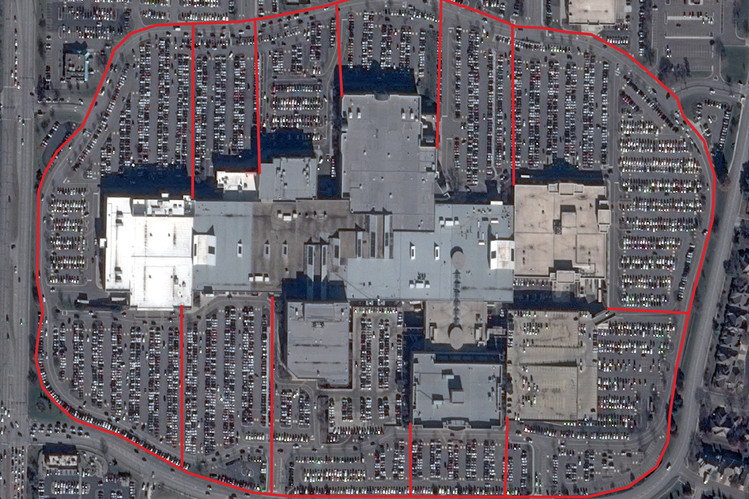
\includegraphics[scale=0.5]{pics/parking_lot.jpg}
 source of image:
https://si.wsj.net/public/resources/images/P1-BO440\_REPLIC\_P\_20131218220538.jpg

During my discussions the topic came up more than once, of converting 1
car/shopper into a better estimate, getting a handle on:

\[total\text{ }shoppers \approx \left(\frac{people}{1{car}}\right)(n_{cars})\]

\subsubsection{Fundalmental Question}\label{fundalmental-question}

\begin{itemize}
\itemsep1pt\parskip0pt\parsep0pt
\item
  How can we better estimate the spending power represented by a car ?
\end{itemize}

\subsubsection{Let's use another proxy}\label{lets-use-another-proxy}

\begin{itemize}
\itemsep1pt\parskip0pt\parsep0pt
\item
  Assume that more people means tendency to higher expenditure
\item
  Bigger vehicle is a more affluent shopper
\item
  Bigger vehicles have the ability to transport more or larger items
\end{itemize}

\subsubsection{How to get vehicle size
estimate}\label{how-to-get-vehicle-size-estimate}

\begin{itemize}
\itemsep1pt\parskip0pt\parsep0pt
\item
  Corner detection on the cars to get vehicle dimension estimates???
\item
  Some other method the CV team can get working.
\end{itemize}

\subsubsection{Experiment}\label{experiment}

\begin{itemize}
\itemsep1pt\parskip0pt\parsep0pt
\item
  We choose a store that is a good candidate for vehicle size detection.
\item
  Calculate vehicle dimension estimates over time
\item
  Assign vehicles to size bins
\item
  Weekends only so that we may assume the whole family is attending
\item
  Obtain gross sales record over 5 years
\item
  Fit sales to car count
\item
  Try to improve fit using vehicle dimensions as an additional parameter
\end{itemize}

    \section{Technical Considerations}\label{technical-considerations}

For simplicity sake: * I'm only using the length dimension * Using an
image sub section with veritcally aligned cars

\subsection{Some vehicle lengths}\label{some-vehicle-lengths}

\begin{itemize}
\itemsep1pt\parskip0pt\parsep0pt
\item
  Chevy Tahoe: $518 cm$
\item
  Toyata Celica: $434 cm$
\end{itemize}

$\Delta{L}=84 cm$

$k_{nyquist}$ for 90 cm camera = 180 cm.

    I estimated the resolution of the satelite image above, by zooming in on
a region with cars. I counted the numebr of pixels that appear to make
up a car and figured that the average car is $\approx 1.7 m$ in width.

    \begin{Verbatim}[commandchars=\\\{\}]
{\color{incolor}In [{\color{incolor}79}]:} \PY{k+kn}{import} \PY{n+nn}{scipy.ndimage}
         \PY{k+kn}{import} \PY{n+nn}{matplotlib.pyplot} \PY{k+kn}{as} \PY{n+nn}{plt}
         \PY{k+kn}{from} \PY{n+nn}{scipy} \PY{k+kn}{import} \PY{n}{fftpack}
         \PY{k+kn}{import} \PY{n+nn}{radialProfile}
         \PY{o}{\PYZpc{}}\PY{k}{matplotlib} inline

         \PY{n}{data} \PY{o}{=} \PY{n}{scipy}\PY{o}{.}\PY{n}{ndimage}\PY{o}{.}\PY{n}{imread}\PY{p}{(}\PY{l+s}{\PYZdq{}}\PY{l+s}{pics/parking\PYZus{}lot.jpg}\PY{l+s}{\PYZdq{}}\PY{p}{,} \PY{n}{flatten}\PY{o}{=}\PY{n+nb+bp}{True}\PY{p}{)}
\end{Verbatim}

    Zoom in enough to count pixels to width. I ount 2 pixels for 1.7 meters

    \begin{Verbatim}[commandchars=\\\{\}]
{\color{incolor}In [{\color{incolor}80}]:} \PY{n}{data\PYZus{}sub} \PY{o}{=} \PY{n}{data}\PY{p}{[}\PY{l+m+mi}{100}\PY{p}{:}\PY{l+m+mi}{200}\PY{p}{,} \PY{l+m+mi}{600}\PY{p}{:}\PY{l+m+mi}{700}\PY{p}{]}
         \PY{n}{plt}\PY{o}{.}\PY{n}{figure}\PY{p}{(}\PY{n}{figsize}\PY{o}{=}\PY{p}{(}\PY{l+m+mi}{10}\PY{p}{,} \PY{l+m+mi}{10}\PY{p}{)}\PY{p}{)}
         \PY{n}{plt}\PY{o}{.}\PY{n}{imshow}\PY{p}{(}\PY{n}{data\PYZus{}sub}\PY{p}{,} \PY{n}{interpolation}\PY{o}{=}\PY{l+s}{\PYZsq{}}\PY{l+s}{nearest}\PY{l+s}{\PYZsq{}}\PY{p}{,} \PY{n}{origin}\PY{o}{=}\PY{l+s}{\PYZsq{}}\PY{l+s}{upper}\PY{l+s}{\PYZsq{}}\PY{p}{,} \PY{n}{cmap}\PY{o}{=}\PY{l+s}{\PYZsq{}}\PY{l+s}{jet}\PY{l+s}{\PYZsq{}}\PY{p}{)}
\end{Verbatim}

            \begin{Verbatim}[commandchars=\\\{\}]
{\color{outcolor}Out[{\color{outcolor}80}]:} <matplotlib.image.AxesImage at 0x7f0485a5e610>
\end{Verbatim}

    \begin{center}
    \adjustimage{max size={0.9\linewidth}{0.9\paperheight}}{idea_number_shoppers_files/idea_number_shoppers_5_1.png}
    \end{center}
    { \hspace*{\fill} \\}

    \subsection{Will A Corner Detection Routine Even
Work?}\label{will-a-corner-detection-routine-even-work}

I don't know\ldots{}maybe. Below is my naive anaylsis of the
feasibility. Boris and Jason can tell us much better.

    \begin{Verbatim}[commandchars=\\\{\}]
{\color{incolor}In [{\color{incolor}81}]:} \PY{k+kn}{import} \PY{n+nn}{sys}
         \PY{n}{sys}\PY{o}{.}\PY{n}{path}\PY{o}{.}\PY{n}{append}\PY{p}{(}\PY{l+s}{\PYZdq{}}\PY{l+s}{/home/daniel/git/Python2.7/DataScience/notebooks/orbital}\PY{l+s}{\PYZdq{}}\PY{p}{)}
\end{Verbatim}

    \begin{Verbatim}[commandchars=\\\{\}]
{\color{incolor}In [{\color{incolor}82}]:} \PY{n}{plt}\PY{o}{.}\PY{n}{figure}\PY{p}{(}\PY{n}{figsize}\PY{o}{=}\PY{p}{(}\PY{l+m+mi}{10}\PY{p}{,} \PY{l+m+mi}{10}\PY{p}{)}\PY{p}{)}
         \PY{n}{plt}\PY{o}{.}\PY{n}{imshow}\PY{p}{(}\PY{n}{data}\PY{p}{,} \PY{n}{interpolation}\PY{o}{=}\PY{l+s}{\PYZsq{}}\PY{l+s}{nearest}\PY{l+s}{\PYZsq{}}\PY{p}{,} \PY{n}{origin}\PY{o}{=}\PY{l+s}{\PYZsq{}}\PY{l+s}{upper}\PY{l+s}{\PYZsq{}}\PY{p}{,} \PY{n}{cmap}\PY{o}{=}\PY{l+s}{\PYZsq{}}\PY{l+s}{jet}\PY{l+s}{\PYZsq{}}\PY{p}{)}
         \PY{n}{plt}\PY{o}{.}\PY{n}{hlines}\PY{p}{(}\PY{l+m+mi}{190}\PY{p}{,} \PY{l+m+mi}{630}\PY{p}{,} \PY{l+m+mi}{680}\PY{p}{,} \PY{l+s}{\PYZsq{}}\PY{l+s}{k}\PY{l+s}{\PYZsq{}}\PY{p}{)}
         \PY{n}{plt}\PY{o}{.}\PY{n}{hlines}\PY{p}{(}\PY{l+m+mi}{140}\PY{p}{,} \PY{l+m+mi}{630}\PY{p}{,} \PY{l+m+mi}{680}\PY{p}{,} \PY{l+s}{\PYZsq{}}\PY{l+s}{k}\PY{l+s}{\PYZsq{}}\PY{p}{)}
         \PY{n}{plt}\PY{o}{.}\PY{n}{vlines}\PY{p}{(}\PY{l+m+mi}{630}\PY{p}{,} \PY{l+m+mi}{140}\PY{p}{,} \PY{l+m+mi}{190}\PY{p}{,} \PY{l+s}{\PYZsq{}}\PY{l+s}{k}\PY{l+s}{\PYZsq{}}\PY{p}{)}
         \PY{n}{plt}\PY{o}{.}\PY{n}{vlines}\PY{p}{(}\PY{l+m+mi}{680}\PY{p}{,} \PY{l+m+mi}{140}\PY{p}{,} \PY{l+m+mi}{190}\PY{p}{,} \PY{l+s}{\PYZsq{}}\PY{l+s}{k}\PY{l+s}{\PYZsq{}}\PY{p}{)}
\end{Verbatim}

            \begin{Verbatim}[commandchars=\\\{\}]
{\color{outcolor}Out[{\color{outcolor}82}]:} <matplotlib.collections.LineCollection at 0x7f0485946350>
\end{Verbatim}

    \begin{center}
    \adjustimage{max size={0.9\linewidth}{0.9\paperheight}}{idea_number_shoppers_files/idea_number_shoppers_8_1.png}
    \end{center}
    { \hspace*{\fill} \\}

    \begin{Verbatim}[commandchars=\\\{\}]
{\color{incolor}In [{\color{incolor}83}]:} \PY{n}{data\PYZus{}sub} \PY{o}{=} \PY{n}{data}\PY{p}{[}\PY{l+m+mi}{140}\PY{p}{:}\PY{l+m+mi}{190}\PY{p}{,} \PY{l+m+mi}{630}\PY{p}{:}\PY{l+m+mi}{680}\PY{p}{]}

         \PY{n}{plt}\PY{o}{.}\PY{n}{figure}\PY{p}{(}\PY{n}{figsize}\PY{o}{=}\PY{p}{(}\PY{l+m+mi}{7}\PY{p}{,} \PY{l+m+mi}{7}\PY{p}{)}\PY{p}{)}
         \PY{n}{plt}\PY{o}{.}\PY{n}{imshow}\PY{p}{(}\PY{n}{data\PYZus{}sub}\PY{p}{,} \PY{n}{interpolation}\PY{o}{=}\PY{l+s}{\PYZsq{}}\PY{l+s}{nearest}\PY{l+s}{\PYZsq{}}\PY{p}{,} \PY{n}{origin}\PY{o}{=}\PY{l+s}{\PYZsq{}}\PY{l+s}{upper}\PY{l+s}{\PYZsq{}}\PY{p}{)}
         \PY{n}{plt}\PY{o}{.}\PY{n}{colorbar}\PY{p}{(}\PY{p}{)}
\end{Verbatim}

            \begin{Verbatim}[commandchars=\\\{\}]
{\color{outcolor}Out[{\color{outcolor}83}]:} <matplotlib.colorbar.Colorbar instance at 0x7f04857d0248>
\end{Verbatim}

    \begin{center}
    \adjustimage{max size={0.9\linewidth}{0.9\paperheight}}{idea_number_shoppers_files/idea_number_shoppers_9_1.png}
    \end{center}
    { \hspace*{\fill} \\}

    \begin{Verbatim}[commandchars=\\\{\}]
{\color{incolor}In [{\color{incolor}84}]:} \PY{k}{def} \PY{n+nf}{fft2D}\PY{p}{(}\PY{n}{data}\PY{p}{)}\PY{p}{:}
             \PY{n}{fft} \PY{o}{=} \PY{n}{fftpack}\PY{o}{.}\PY{n}{fft2}\PY{p}{(}\PY{n}{data}\PY{p}{)}
             \PY{n}{fft\PYZus{}shift} \PY{o}{=} \PY{n}{fftpack}\PY{o}{.}\PY{n}{fftshift}\PY{p}{(}\PY{n}{fft}\PY{p}{)}
             \PY{n}{power2D} \PY{o}{=} \PY{n}{np}\PY{o}{.}\PY{n}{abs}\PY{p}{(}\PY{n}{fft\PYZus{}shift}\PY{p}{)}\PY{o}{*}\PY{o}{*}\PY{l+m+mi}{2}
             \PY{n}{power1D} \PY{o}{=} \PY{n}{radialProfile}\PY{o}{.}\PY{n}{azimuthalAverage}\PY{p}{(}\PY{n}{power2D}\PY{p}{)}

             \PY{k}{return} \PY{n}{power1D}
\end{Verbatim}

    \begin{Verbatim}[commandchars=\\\{\}]
{\color{incolor}In [{\color{incolor}88}]:} \PY{c}{\PYZsh{}\PYZsh{} k space scale}
         \PY{k}{def} \PY{n+nf}{k\PYZus{}scale}\PY{p}{(}\PY{n}{dim}\PY{p}{,} \PY{n}{npts}\PY{p}{)}\PY{p}{:}
             \PY{n}{camera\PYZus{}res} \PY{o}{=} \PY{l+m+mi}{90} \PY{c}{\PYZsh{} cm           }
             \PY{n}{max\PYZus{}len} \PY{o}{=} \PY{n}{camera\PYZus{}res} \PY{o}{*} \PY{n}{dim} \PY{c}{\PYZsh{}cm , size of sub plot}
             \PY{n}{nyq} \PY{o}{=} \PY{l+m+mi}{2} \PY{o}{*} \PY{l+m+mi}{90} \PY{c}{\PYZsh{}cm}
             \PY{n}{range\PYZus{}} \PY{o}{=} \PY{n}{max\PYZus{}len} \PY{o}{\PYZhy{}} \PY{n}{nyq}
             \PY{c}{\PYZsh{} reverse order}
             \PY{n}{k} \PY{o}{=} \PY{n}{np}\PY{o}{.}\PY{n}{flipud}\PY{p}{(}\PY{n}{np}\PY{o}{.}\PY{n}{arange}\PY{p}{(}\PY{n}{nyq}\PY{p}{,} \PY{n}{max\PYZus{}len}\PY{p}{,}\PY{n}{range\PYZus{}}\PY{o}{/}\PY{n}{npts}\PY{p}{)}\PY{p}{)}
             \PY{k}{return} \PY{n}{k}
\end{Verbatim}

    \begin{Verbatim}[commandchars=\\\{\}]
{\color{incolor}In [{\color{incolor}90}]:} \PY{n}{power1D} \PY{o}{=} \PY{n}{fft2D}\PY{p}{(}\PY{n}{data\PYZus{}sub}\PY{p}{)}
         \PY{n}{k} \PY{o}{=} \PY{n}{k\PYZus{}scale}\PY{p}{(}\PY{n}{data\PYZus{}sub}\PY{o}{.}\PY{n}{shape}\PY{p}{[}\PY{l+m+mi}{0}\PY{p}{]}\PY{p}{,} \PY{n}{power1D}\PY{o}{.}\PY{n}{shape}\PY{p}{[}\PY{l+m+mi}{0}\PY{p}{]}\PY{p}{)}

         \PY{n}{plt}\PY{o}{.}\PY{n}{figure}\PY{p}{(}\PY{n}{figsize}\PY{o}{=}\PY{p}{(}\PY{l+m+mi}{10}\PY{p}{,} \PY{l+m+mi}{5}\PY{p}{)}\PY{p}{)}
         \PY{n}{plt}\PY{o}{.}\PY{n}{plot}\PY{p}{(}\PY{n}{k}\PY{p}{[}\PY{l+m+mi}{1}\PY{p}{:}\PY{p}{]}\PY{p}{,} \PY{n}{power1D}\PY{p}{)}
         \PY{n}{plt}\PY{o}{.}\PY{n}{grid}\PY{p}{(}\PY{p}{)}
\end{Verbatim}

    \begin{center}
    \adjustimage{max size={0.9\linewidth}{0.9\paperheight}}{idea_number_shoppers_files/idea_number_shoppers_12_0.png}
    \end{center}
    { \hspace*{\fill} \\}

    Try again with an edge filter first.

    \begin{Verbatim}[commandchars=\\\{\}]
{\color{incolor}In [{\color{incolor}91}]:} \PY{n}{sobel} \PY{o}{=} \PY{n}{scipy}\PY{o}{.}\PY{n}{ndimage}\PY{o}{.}\PY{n}{filters}\PY{o}{.}\PY{n}{sobel}\PY{p}{(}\PY{n}{data}\PY{p}{)}
         \PY{n}{sobel\PYZus{}sub} \PY{o}{=} \PY{n}{sobel}\PY{p}{[}\PY{l+m+mi}{140}\PY{p}{:}\PY{l+m+mi}{190}\PY{p}{,} \PY{l+m+mi}{630}\PY{p}{:}\PY{l+m+mi}{680}\PY{p}{]}
         \PY{n}{sobel\PYZus{}sub}\PY{p}{[}\PY{n}{np}\PY{o}{.}\PY{n}{isnan}\PY{p}{(}\PY{n}{sobel\PYZus{}sub}\PY{p}{)}\PY{p}{]} \PY{o}{=} \PY{l+m+mi}{0}
         \PY{c}{\PYZsh{}sobel\PYZus{}sub = np.abs(sobel\PYZus{}sub) \PYZsh{} bad idea}

         \PY{n}{plt}\PY{o}{.}\PY{n}{figure}\PY{p}{(}\PY{n}{figsize}\PY{o}{=}\PY{p}{(}\PY{l+m+mi}{7}\PY{p}{,} \PY{l+m+mi}{7}\PY{p}{)}\PY{p}{)}
         \PY{n}{plt}\PY{o}{.}\PY{n}{imshow}\PY{p}{(}\PY{n}{sobel\PYZus{}sub}\PY{p}{,} \PY{n}{interpolation}\PY{o}{=}\PY{l+s}{\PYZsq{}}\PY{l+s}{nearest}\PY{l+s}{\PYZsq{}}\PY{p}{,} \PY{n}{origin}\PY{o}{=}\PY{l+s}{\PYZsq{}}\PY{l+s}{upper}\PY{l+s}{\PYZsq{}}\PY{p}{)}
         \PY{n}{plt}\PY{o}{.}\PY{n}{colorbar}\PY{p}{(}\PY{p}{)}
\end{Verbatim}

            \begin{Verbatim}[commandchars=\\\{\}]
{\color{outcolor}Out[{\color{outcolor}91}]:} <matplotlib.colorbar.Colorbar instance at 0x7f0486df5fc8>
\end{Verbatim}

    \begin{center}
    \adjustimage{max size={0.9\linewidth}{0.9\paperheight}}{idea_number_shoppers_files/idea_number_shoppers_14_1.png}
    \end{center}
    { \hspace*{\fill} \\}

    \begin{Verbatim}[commandchars=\\\{\}]
{\color{incolor}In [{\color{incolor}92}]:} \PY{n}{power1D\PYZus{}sobel} \PY{o}{=} \PY{n}{fft2D}\PY{p}{(}\PY{n}{sobel\PYZus{}sub}\PY{p}{)}
         \PY{n}{plt}\PY{o}{.}\PY{n}{figure}\PY{p}{(}\PY{n}{figsize}\PY{o}{=}\PY{p}{(}\PY{l+m+mi}{10}\PY{p}{,} \PY{l+m+mi}{5}\PY{p}{)}\PY{p}{)}
         \PY{n}{plt}\PY{o}{.}\PY{n}{plot}\PY{p}{(}\PY{n}{k}\PY{p}{[}\PY{l+m+mi}{1}\PY{p}{:}\PY{p}{]}\PY{p}{,} \PY{n}{power1D\PYZus{}sobel}\PY{p}{)}
         \PY{n}{plt}\PY{o}{.}\PY{n}{grid}\PY{p}{(}\PY{p}{)}
\end{Verbatim}

    \begin{center}
    \adjustimage{max size={0.9\linewidth}{0.9\paperheight}}{idea_number_shoppers_files/idea_number_shoppers_15_0.png}
    \end{center}
    { \hspace*{\fill} \\}

    \section{Conclusion}\label{conclusion}
    I'm hoping that the roughly 2, 3 and 3.5 meter peaks are cars and that
means we can classify vehicles by size.


    % Add a bibliography block to the postdoc



    \end{document}
